\subsection{Optimization: Stochastic Gradient Descent (SGD)}
Eine alternative \textbf{Optimierungsfunktion} SGD.\\
\textbf{Error-Function der linearen Gleichung:}
$$E = \frac{1}{2N} \sum_{i=1}^N e^2_i =\frac{1}{2N} \sum_{i=1}^N (y_i - (a*x_i+b))^2$$
\begin{itemize}
\item \textbf{Gradient} (in Vektor Ableitung nach \textbf{a} und einmal nach \textbf{b} und dies in einem Vektor platzieren
    $$ Gradient \: of \: E =$$
    $$\begin{bmatrix}
       \frac{\delta E}{\nabla a} \\
       \frac{\delta E}{\nabla b} \\
     \end{bmatrix}
         = 
    \begin{bmatrix}
    \frac{1}{N} \sum_{i=1}^N (y_i - (a * x_i + b))(-x_i) \\
       \frac{\delta E}{\nabla b}(y_i - (a * x_i + b))(-1) \\
     \end{bmatrix}
    $$
\end{itemize}
Problem hier: Der normale Gradient dient dazu von einem Tal auf einen Berg zu kommen, also vom Minimum zum Maximum, zudem macht er noch zu grosse Schritte (Bild 1). Dies läsen wir indem wir noch ein alpha hinzufügen und die Werte negieren (Bild 2):
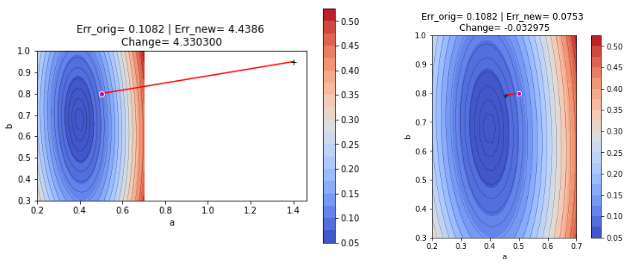
\includegraphics[width=\linewidth]{img/gradient_schritt.png}
Um nun weiterzukommen und immer näher ins Tal zu kommen zum minimalen Error, müssen wir nun am neuen Punkt wieder den Gradient berechnen:
\\
    $\begin{bmatrix}
       a \\
       b \\
    \end{bmatrix}_{t+1}
     = 
    \begin{bmatrix}
       a \\
       b \\
    \end{bmatrix}_{t}
     - \alpha     
    \begin{bmatrix}
       \frac{\delta E}{\nabla a} \\
       \frac{\delta E}{\nabla b} \\
    \end{bmatrix}
    |_{
    \begin{bmatrix}
       a \\
       b \\
    \end{bmatrix}_t
    }
    $
\\
Dies geht so lange weiter bis man eine bestimmte Anzahl Iterationen erreicht hat, die vorgegeben wird. Daraus ergibt sich eine Learning-Kurve. In diesem Beispiel ist schon nach 20 iterationen das Ziel beinahe erreicht und nur noch am b wird optimiert.
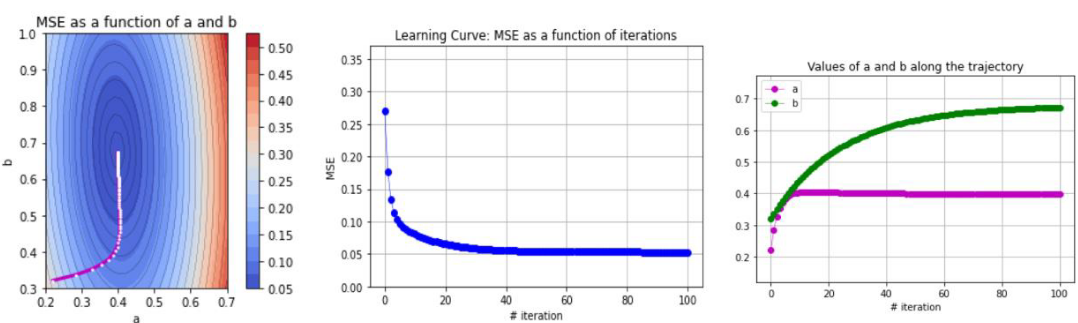
\includegraphics[width=\linewidth]{img/gradient_learning_curve.png}
\textit{Hinweis: Hat man mehr als ein Tal, dann muss man einfach an mehreren Punkten starten und so versuchen das Globale Minimum zu finden (Mehrere Punkte unterschiedliches Minimum, dann den tiefsten nehmen)}\\\
\textbf{Hier noch ein Bild, welches die Idee noch veranschaulicht:}\\
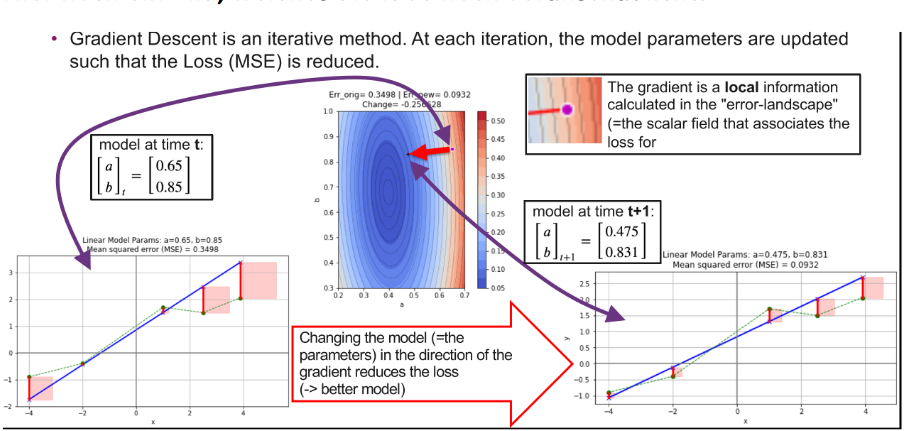
\includegraphics[height=0.7\linewidth, angle=90]{img/gradient_explanation.png}
\subsection{Stochastic Gradient Descent (SGD)}
SGD hilft das (lokale) Minimum zu finden. Man startet random an verschiedenen Punkten, damit die Chance das globale Minimum zu finden grösser ist. In jedem Schritt wird der\textbf{ ganze Parametervektor} optimiert.
Hier ist das Ziel, dass man nur eine kleine Menge and Datenpunkte nimmt um die Fehler und so den Gradient zu berechnen. Man selektiert also random ein paar Datenpunkte aus dem Dataset (J = Teildatenset):
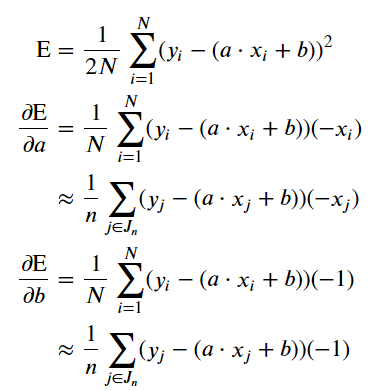
\includegraphics[width=0.7\linewidth]{img/sgd_formula.png}\\
Dies führt zur folgender Update-Regel mit welcher man den Parametervektor berechnen kann (bei uns musste nie abgeleitet werden und das Ableitungszeichen konnte ignoriert werden):
    $$\begin{bmatrix}
       a \\
       b \\
    \end{bmatrix}_{t+1}
     = 
    \begin{bmatrix}
       a \\
       b \\
    \end{bmatrix}_{t}
     - \alpha     
    \begin{bmatrix}
       \frac{\delta E}{\nabla a} \\
       \frac{\delta E}{\nabla b} \\
    \end{bmatrix}
    |_{
    \begin{bmatrix}
       a \\
       b \\
    \end{bmatrix}_t
    }
    $$
Nun versucht man den Batch auf 1 zu wählen oder möglichst klein (32 oder 64 werden häufig verwendet).\\
\textit{Hinweis: Bei Batch 1 kann es sehr grosse Zicksacke geben, da ja für einen Punkt mehr als eine Lösung gibt und MSE auch 0 sein kann. Dennoch kommt man irgendwann auf eine Lösung, doch es gibt Zickzackwerte bei der Lerning-Kurve. Und nahe beim Ziel geht er wieder weiter weg. Dieses Problem kann aber auch gelöst werden indem man Alpha immer kleiner wählt.}
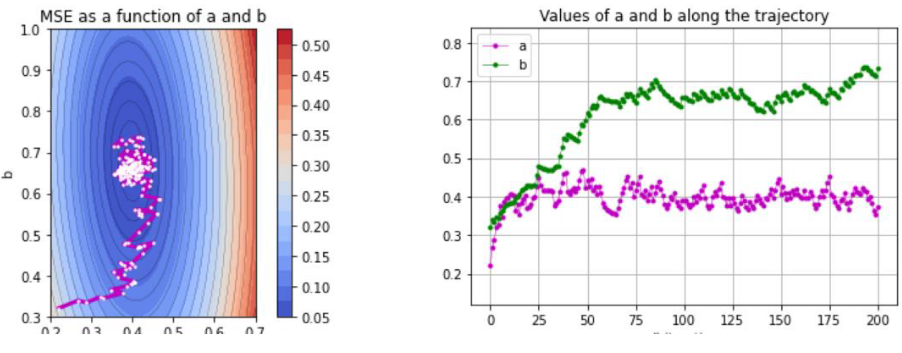
\includegraphics[width=\linewidth]{img/sgd_learning_curve.png}
\subsection{Stochastic Gradient Descent with annealed learning rate}
Wie oben erwähnt gibt es eine grosse Streuung am Ende und man erreicht nicht mehr so genaue Werte. Dem kann man entgegenwirken indem man immer alle paar Iterationen alpha(Lernrate) verkleinert. Somit flacht es nach ein paar Iterationen immer mehr aus und man kommt anfangs sehr schnell in die Mitte:
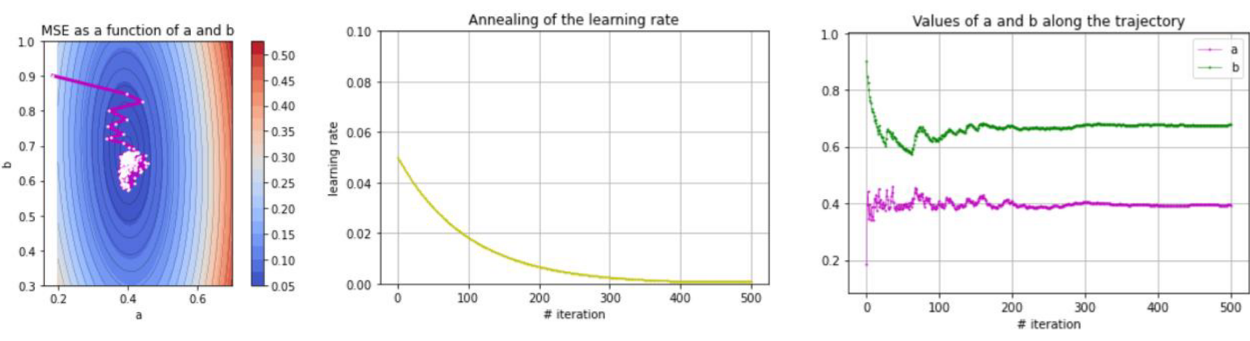
\includegraphics[width=\linewidth]{img/sgd_annealed_learning_curve.png}

\subsection{Allgemeine Anmerkungen}
\begin{itemize}
\item Diese Methode geht nur, wenn die Loss-Function ableitbar ist.
\item SGD kann nur mit einem Datenset arbeiten, was sehr ineffizient ist und selten benutzt wird
\begin{itemize}
\item Batch oder Minibatch-Gradient ist also besser
\end{itemize}
\item SGD muss der Gradient berechnen. Ist dies schwer?
\begin{itemize}
\item Ja, wenn man es selbst tun muss und es viele Parameter gibt. (Neurale Netze können Millionen Parameter haben)
\item Nein, wenn man ein Modell hat und ein Machine Learning Framework nutzt (Tensorflow, Pytorch).
\end{itemize}
\item Gradient Descent ist ein Basis Baustein für viele weitere Algorithmen wie Adam, Adagrad, RMSProp, etc.
\end{itemize}
